\usetikzlibrary {arrows.meta, shapes.geometric, positioning}
\newcommand{\hdist}{1.25cm}
\newcommand{\vdist}{0.8cm}

\begin{landscape}
    \section{Power Distribution Block Diagram}
    \vfill
    \center
    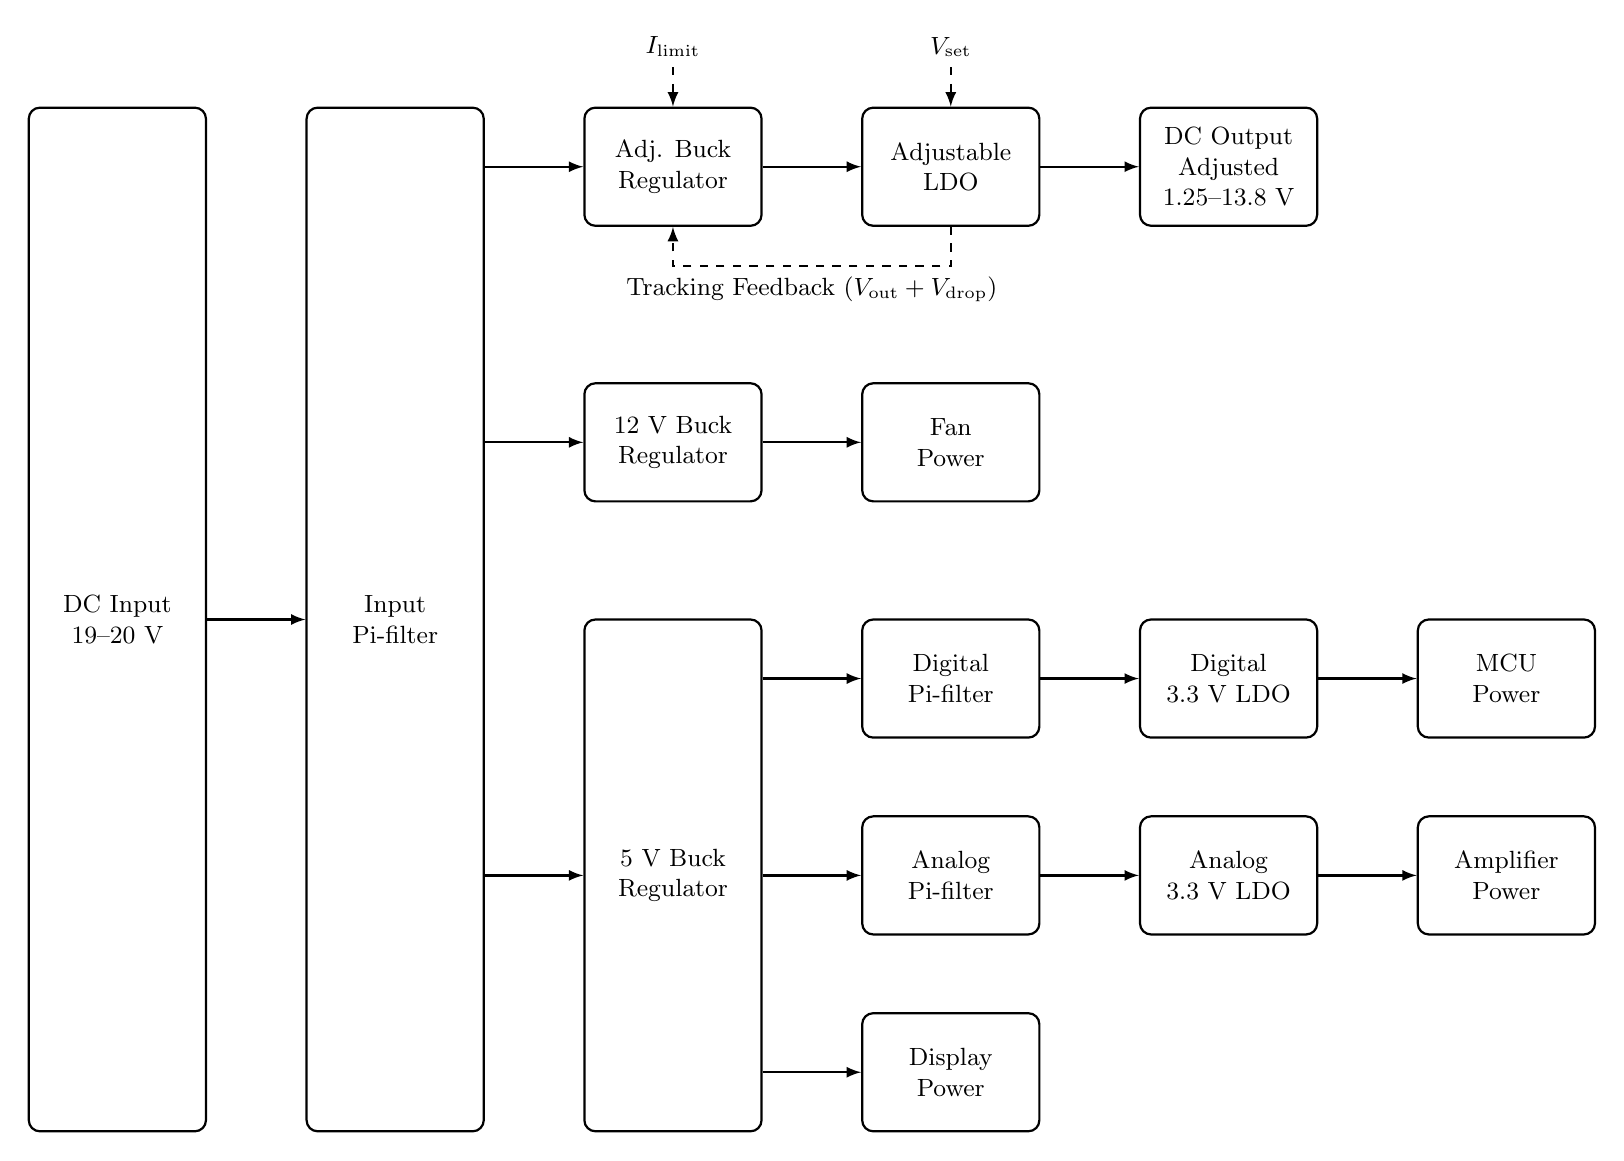
\begin{tikzpicture}[
        node distance=\vdist and \hdist,
        >=latex,
        thick,
        every node/.style={draw, minimum width=2.25cm, rounded corners, align=center, font=\small},
    ]
        \node[minimum height=13cm] (input) {DC Input\\19--20 V};
        \node[minimum height=13cm,right=of input] (input_filter) {Input\\Pi-filter};
        \draw[->] (input) -- (input_filter);

        \coordinate (x)       at ([yshift= 2.25cm]input_filter.east);
        \coordinate (x_north) at ([yshift= 5.75cm]input_filter.east);
        \coordinate (x_south) at ([yshift=-3.25cm]input_filter.east);
        \node[minimum height=1.5cm, right=of x]       (buck_12v) {12 V Buck\\ Regulator};
        \node[minimum height=1.5cm, right=of x_north] (buck_adj) {Adj. Buck\\Regulator};
        \node[minimum height=6.5cm, right=of x_south] (buck_5v)  {5 V Buck\\ Regulator};
        \draw[->] (x)       -- (buck_12v);
        \draw[->] (x_north) -- (buck_adj);
        \draw[->] (x_south) -- (buck_5v);

        \coordinate (x)       at (buck_5v.east);
        \coordinate (x_north) at ([yshift= 2.5cm]buck_5v.east);
        \coordinate (x_south) at ([yshift=-2.5cm]buck_5v.east);
        \node[minimum height=1.5cm, right=of x]       (analog_filter)  {Analog\\Pi-filter};
        \node[minimum height=1.5cm, right=of x_north] (digital_filter) {Digital\\Pi-filter};
        \node[minimum height=1.5cm, right=of x_south] (display)        {Display\\Power};
        \draw[->] (x)       -- (analog_filter);
        \draw[->] (x_north) -- (digital_filter);
        \draw[->] (x_south) -- (display);        

        \node[minimum height=1.5cm, right=of buck_12v] (fan) {Fan\\Power};
        \draw[->] (buck_12v) -- (fan);

        \node[minimum height=1.5cm, right=of analog_filter]  (analog_ldo)  {Analog\\3.3 V LDO};
        \node[minimum height=1.5cm, right=of digital_filter] (digital_ldo) {Digital\\3.3 V LDO};
        \draw[->] (analog_filter)  -- (analog_ldo);
        \draw[->] (digital_filter) -- (digital_ldo);

        \node[minimum height=1.5cm, right=of analog_ldo]  (amplifier) {Amplifier\\Power};
        \node[minimum height=1.5cm, right=of digital_ldo] (mcu)       {MCU\\Power};
        \draw[->] (analog_ldo)  -- (amplifier);
        \draw[->] (digital_ldo) -- (mcu);

        \node[minimum height=1.5cm, right=of buck_adj] (ldo_adj) {Adjustable\\LDO};
        \node[minimum height=1.5cm, right=of ldo_adj]  (output)  {DC Output\\Adjusted\\1.25--13.8 V};
        \draw[->] (buck_adj) -- (ldo_adj);
        \draw[->] (ldo_adj) -- (output);

        \coordinate (a) at ([yshift=-0.5cm]ldo_adj.south);
        \coordinate (b) at ([yshift=-0.5cm]buck_adj.south);
        \draw[->, dashed] (ldo_adj) -- (a) -- node[draw=none, below]{Tracking Feedback ($V_\mathrm{out}+V_\mathrm{drop}$)}(b) -- (buck_adj);
        \coordinate (a) at ([yshift= 0.5cm]ldo_adj.north);
        \coordinate (b) at ([yshift= 0.5cm]buck_adj.north);
        \draw[->, dashed] (a) node[draw=none, above]{$V_\mathrm{set}$} -- (ldo_adj.north);
        \draw[->, dashed] (b) node[draw=none, above]{$I_\mathrm{limit}$} -- (buck_adj.north);
    \end{tikzpicture}
    \vfill
\end{landscape}